%!TEX encoding = UTF-8 Unicode

\documentclass[code,math]{relatorio-deti}

\title{HW1: Mid-term assignment report}
\cadeira{Software Testing and Quality Control}
\relatorioAno{2024/2025}

\membro{Duarte Gabriel Castro Branco}{119253}

\usepackage{lmodern}
\usepackage{lipsum}
\usepackage{tocloft}
\usepackage{wasysym}

\begin{document}

\maketitle

\tableofcontents
\clearpage


\pagenumbering{arabic}
\chapter{Introduction}
\section{Overview of the work}

This report presents the midterm individual project developed for the \textit{Teste e Qualidade de Software} (TQS) course. This project, \texttt{ZeroMonos}, is a simple full-stack web app designed for a fictional waste management company that provides a garbage collection service in multiple municipalities. The system should allow citizens to book this service, by picking a date, their municipality and the type and description of the items they want to get rid of. It should also allow for staff to manage these bookings.

The system exposes a Spring Boot REST API and a \texttt{Thymeleaf} web app for the front-end. It supports both citizen and staff facing interactions and integrates a complete automated testing strategy (unit, service, integration, function, performance and code quality analysis).

\section{Current implementation (faults \& extras)}

All core function requirements from the assignment were implemented:

\begin{itemize}
    \item Citizens can create bookings specifying their name, municipality, date and item description.
    \item Municipalities are dynamically fetched from an external API (\href{https://json.geoapi.pt/municipios}{https://json.geoapi.\linebreak pt/municipios}).
    \item Upon successful booking, the citizen gets a unique token with which he can check the request's state and even cancel it.
    \item Bookings are persisted in a \texttt{PostgreSQL} database.
    \item Staff can view, update and delete existing bookings, as well as browse for existing requests, per municipality.
\end{itemize}

In addition to the required functionalities, the project integrates a \texttt{Continuous Integration (CI)} pipeline using GitHub Actions. It's set up to build and test the project on each push/merge request, and it includes \texttt{SonarQube} Quality Gate enforcement via \texttt{SonarQube Cloud}.

Yet, the current implementation has some constraints and missing features, such as mobile responsiveness and an authentication/login system.

\chapter{Product specification}
\section{Functional scope and supported interactions}

The \texttt{ZeroMonos} platform is designed for two primary actor types:

\begin{itemize}
	\item \textbf{Citizens}: Regular users who want to dispose of bulky waste.
	\item  \textbf{Staff}: Authorized personnel who oversee and manage the collection requests.
\end{itemize}

Each actor interacts with the system in different ways.

The citizen has these main interactions:

\begin{itemize}
    \item \textbf{Create a Booking}: The citizen fills out a form with their name, selects their municipality from a list and describes the items to be collected (type and description). Upon submission, the system records the booking in the database and generates a unique token, which is displayed to the user. This token acts as a key for later tracking.
    \item \textbf{Check Booking}: Using the token received, the citizen can navigate to a status page and input the token to retrieve the current status of their request. Optionally, the user can also cancel the booking.
\end{itemize}

The staff has these main interactions:

\begin{itemize}
    \item \textbf{Manage bookings}: The staff can view and edit the bookings created by the users. He has the ability to change the initial state of each booking (RECEIVED) to any of these: ASSIGNED (when someone has been assigned to take care of that booking), IN\_PROGRESS (when the booking is being taken care of right now) and COMPLETED. Also, the booking can be completely removed.
    \item \textbf{Filter by Municipality}: The staff can also filter the bookings list by municipality name. This is useful if the system is full of bookings from everywhere, making the managing process easier. The interface provides a search input where staff can type the municipality (e.g. "Aveiro") and the list updates to show only matching bookings.
\end{itemize}

\begin{figure}[ht]
    \centering
    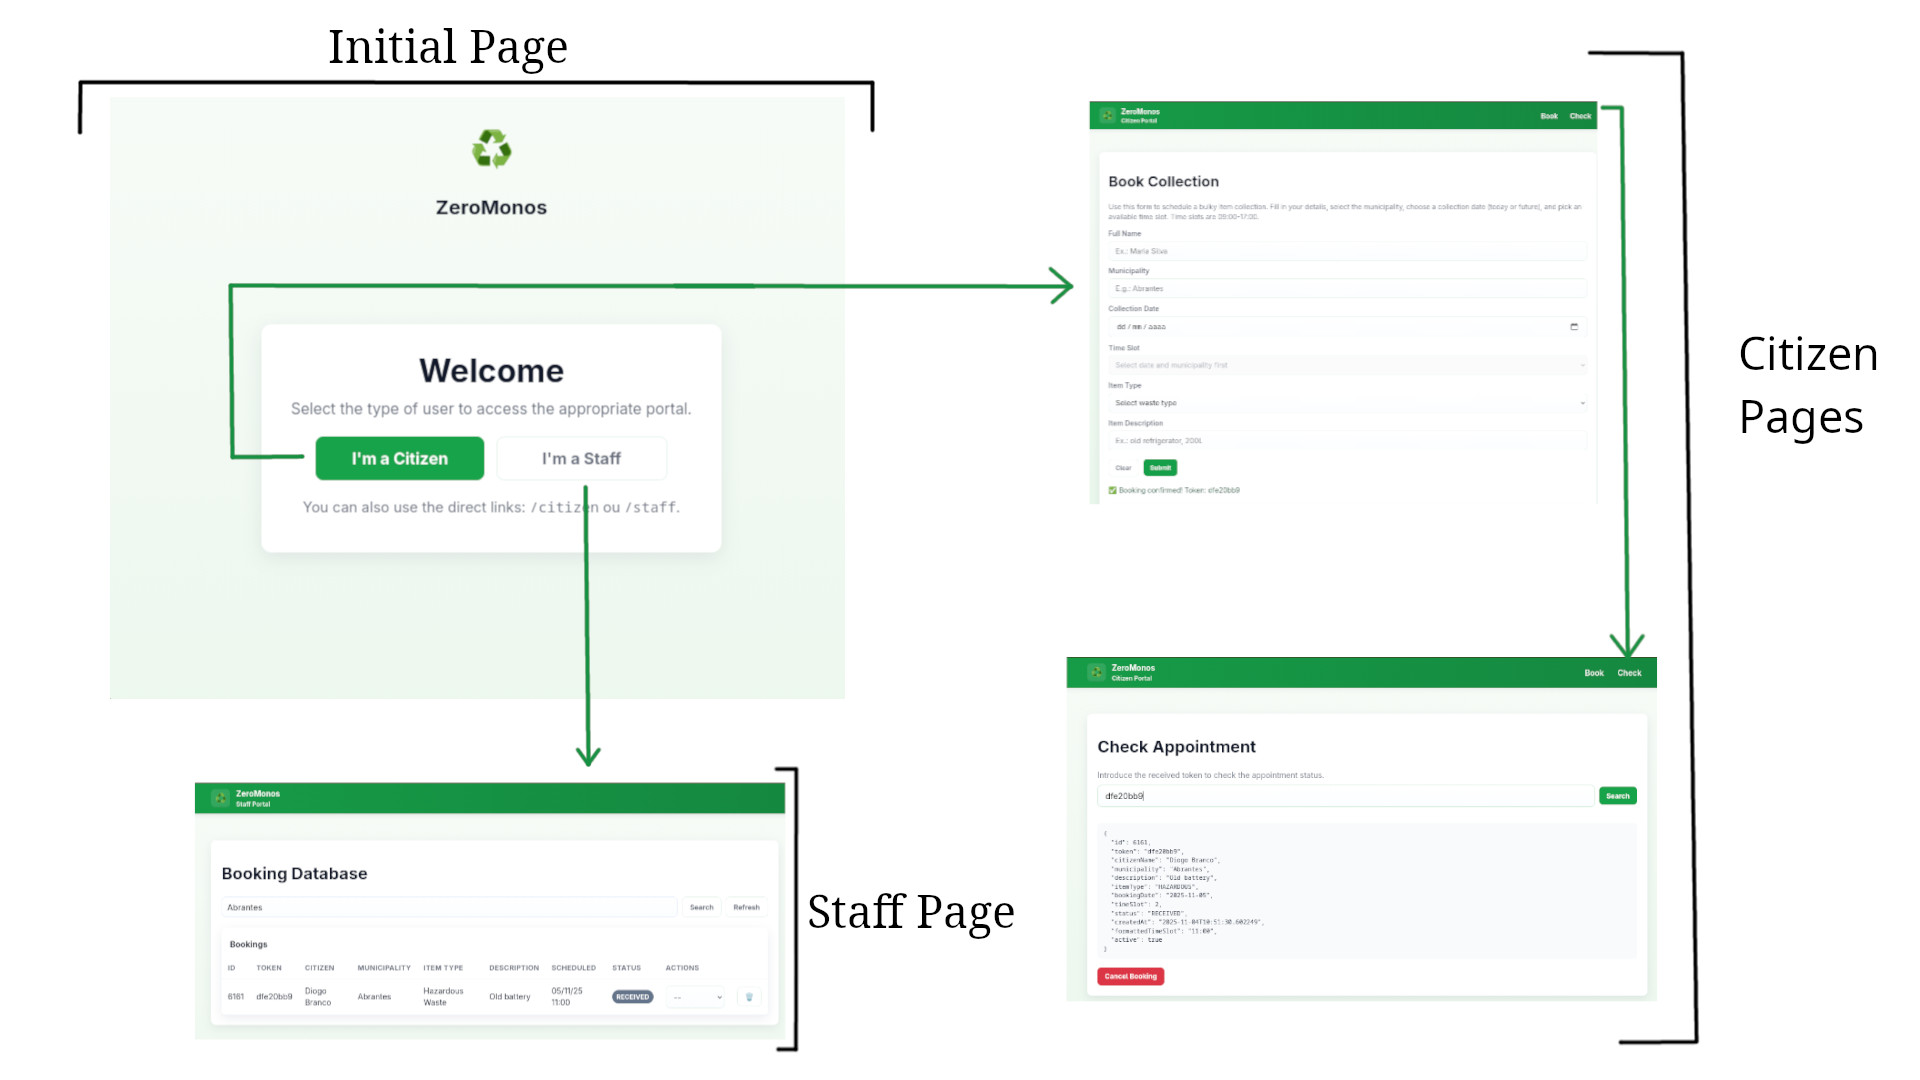
\includegraphics[width=0.8\textwidth]{images/interactions.jpg}
    \caption{Overview of the \texttt{ZeroMonos} application flow}
\end{figure}

\section{System implementation architecture}

\texttt{ZeroMonos} follows a standard Spring Boot web application architecture with a layered structure:

\begin{itemize}
    \item \textbf{Back-End}: The core is a Spring Boot application (Java) that exposes both \texttt{RESTful} endpoints and serves web pages. It uses a service/business layer to implement business logic (for example generating tokens, handling status changes, etc.) and a repository/persistence layer to interact with the database. Data is stored in a \texttt{PostgreSQL} database. The main data entity is the \texttt{Booking.java} which has fields for ID, token, citizen name, municipality, description, status, etc.
    \item \textbf{Front-End}: The web front-end is built using \texttt{Thymeleaf} templates, which are served by Spring Boot controllers. The base structure and navigation are defined in \texttt{layout.html}, which provides common fragments for the header, footer, and scripts in all other pages (\texttt{index.html}, \texttt{citizen-reserve.html}, \texttt{citizen-check.html} and \texttt{staff.html}). Styling is handled by \texttt{style.css}, which defines a clean and responsive visual design. Interactivity is implemented through three JavaScript modules: \texttt{layout.js} (manages shared UI behavior), \texttt{citizen.js} (handles all requests to the API needed for the citizen-facing pages) and \texttt{staff.js} (handles API interactions for the staff-facing page).
\end{itemize}

\begin{figure}[ht]
    \centering
    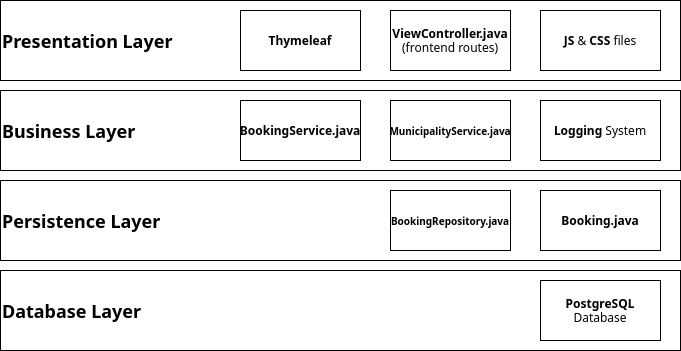
\includegraphics[width=0.8\textwidth]{images/zeromonos_arch.png}
    \caption{Layered architecture of \texttt{ZeroMonos}}
\end{figure}

The app also integrates with an external API for Portuguese municipalities. The application fetches the list of all municipalities by calling the \texttt{geoapi.pt} service (specifically, an endpoint providing a \texttt{JSON} list of municipalities). This is done via a Spring \texttt{RestTemplate} call in a \texttt{MunicipalityService} component. On first use, the service retrieves the list of municipality names and caches them in memory for faster usage later. Docker is also used to create the instance of a local \texttt{PostgreSQL} database.

\section{API for developers}
\label{sec:apifordevelopers}

\texttt{ZeroMonos} provides a REST API that allows external clients to interact with the system. All endpoints use \texttt{JSON} for requests and responses. The key API endpoints include:

\begin{itemize}
	% citizen
    \item \textbf{POST /bookings} - Create a new booking request. The request body should contain the necessary booking details.
    \item \textbf{GET /bookings/\{token\}} - Retrieve an existing booking by its public token. This is intended for the check page to fetch the current details and status of their request.

	% staff
    \item \textbf{GET /bookings} - Retrieve all bookings in the system. This returns a list of all Booking records (intended for staff). This endpoint also supports query parameters (e.g. GET /bookings?municipality=Aveiro\&?date=2025-11-05) to filter the results by municipality and current date.
    \item \textbf{DELETE /bookings/\{id\}} - Remove a booking record (staff use). This permanently deletes the booking with the given internal ID from the database.
    \item \textbf{PATCH /bookings/\{id\}?status=\{newStatus\}} - Update the state of a booking (staff use). The \{id\} in the URL is the internal ID of the booking and \{newStatus\} is the new state.

    \item \textbf{GET /bookings/available-slots} - Returns a list of available time slots for a specific date and municipality, according to the bookings already set up on that day and municipality.
    \item \textbf{GET /municipalities} - Gets the municipalities names from other API. It has a fallback in case the \texttt{geoapi.pt} returns nothing or something invalid.
\end{itemize}

These endpoints make it possible to interact with \texttt{ZeroMonos} from other front-ends or integrate it into a larger platform.

\begin{figure}[ht]
    \centering
    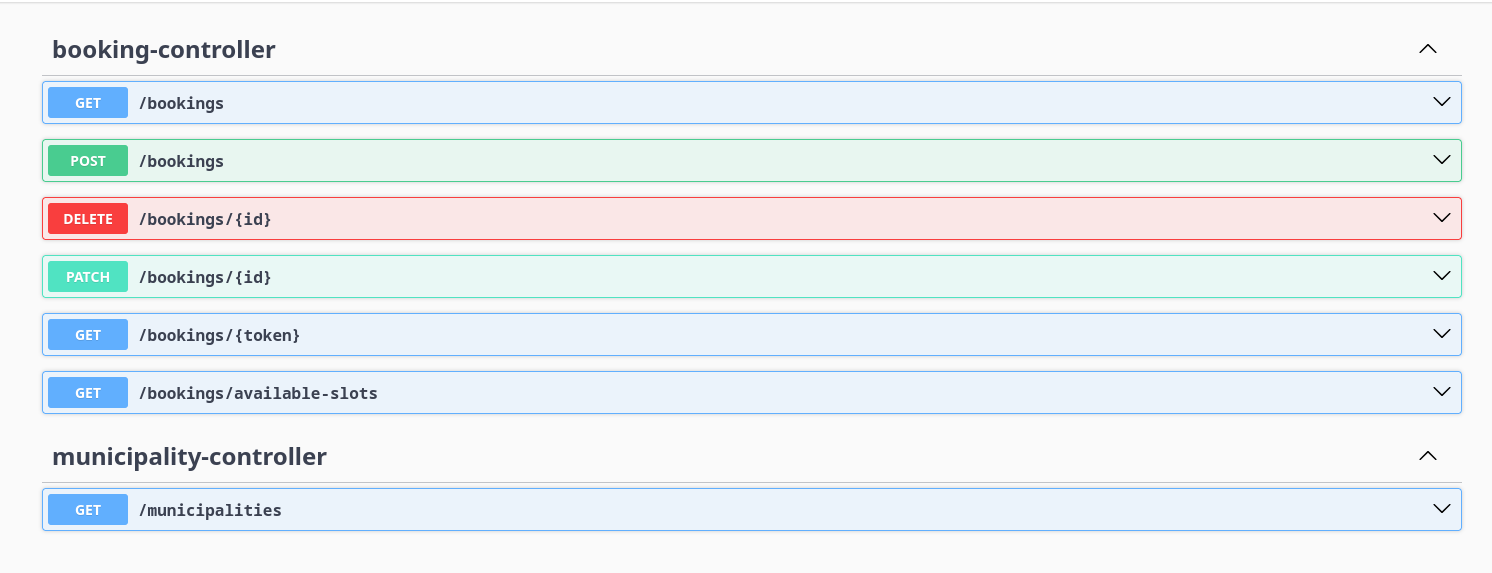
\includegraphics[width=0.8\textwidth]{images/endpoints.png}
    \caption{Swagger UI screenshot}
\end{figure}

\chapter{Quality assurance}
\section{Overall strategy for testing}

The project adopted a layered testing strategy combining \textbf{unit tests}, \textbf{service tests} , \textbf{integration tests}, \textbf{functional tests}, and \textbf{performance simulations}.

The tests rely on \texttt{JUnit 5} and \texttt{Mockito} for unit and service tests, and use Spring’s \texttt{MockMvc} for API integration testing. \texttt{Selenium WebDriver} enabled BDD-style UI automation tests. Finally, non-functional testing was implemented using \texttt{k6} scripts to stress-test the app.

For code analysis, a CI pipeline integrated with \texttt{SonarQube Cloud} was used.

\section{Unit and integration testing}

Unit tests were used extensively for core business logic, particularly within \texttt{Boo\linebreak kingService} and \texttt{MunicipalityService}. These tests validated \textbf{date and slot constraints}, \textbf{status transitions}, \textbf{token-based queries}, and \textbf{fallback behavior} for external APIs.

\begin{itemize}
  \item \textbf{BookingServiceTest:} verifies key domain constraints, including:
  \begin{itemize}
    \item A booking can only be created if the slot is free and the input is valid.
    \item Status transitions (e.g., to \texttt{IN\_PROGRESS} or \texttt{CANCELLED}) are correctly persisted.
    \item Filtering methods work as expected for date, token, and municipality.
  \end{itemize}

  \item \textbf{MunicipalityServiceTest:} handles the geo API and tests the fallback behavior
\end{itemize}

Integration tests leverage Spring Boot's \texttt{@SpringBootTest} and \textit{MockMvc} to test real HTTP interactions and application state via the controllers. Scenarios covered include all the main REST operations from the defined API (see Section~\ref{sec:apifordevelopers}).

\begin{itemize}
  \item \textbf{BookingControllerTest} validates all booking related API flows.

  \item \textbf{MunicipalityControllerTest} validates the return of the municipalities list.
\end{itemize}

Additionally, domain-level validation was tested in \texttt{BookingValidationTest}, ensuring that entity constraints on fields like name, description, item type, and time slot conform to validation rules. These tests catch input issues before persistence or logic execution.

\section{Acceptance testing}

The end-user functionality was tested using Selenium WebDriver in a BDD-like style. Firefox was used in headless mode for full-stack tests involving the booking and status-checking UI. These functional tests (\texttt{FunctionalSeleniumTest}) are written using the Page Object Model (\texttt{BookReservePage}, \texttt{CitizenCheckPage}, \texttt{StaffPage}) and cover the following workflows:

\begin{itemize}
  \item Citizen successfully books two collection slots in different municipalities.
  \item Staff views that newly created bookings and updates it's state.
  \item Staff filters the bookings by municipality, seeing them both separately.
  \item Citizen checks booking status using a token and cancels it.
\end{itemize}

Tests were executed sequentially, reusing state between steps when necessary, and included verification of UI changes and database effects.

I also generated a \texttt{Lighthouse} report for the initial web page and got very high scores (see Fig~\ref{fig: lighthousereport}).

\begin{figure}[ht]
    \centering
    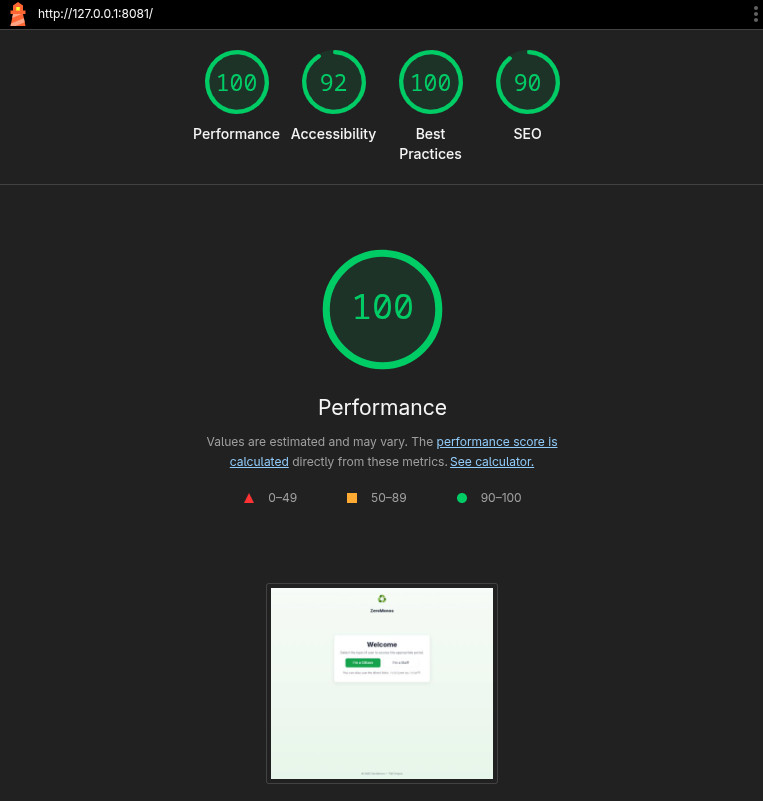
\includegraphics[width=0.8\textwidth]{images/lighthousereport.jpg}
    \caption{Lighthouse report}
	\label{fig: lighthousereport}
\end{figure}

\section{Non-functional testing}

Performance and load testing was carried out using \texttt{k6}. Three scenarios were tested against the \texttt{POST /bookings} endpoint:

\begin{itemize}
  \item \textbf{Baseline load} (\texttt{performance.js}): simulates standard traffic to verify stable response times and success rate.
  \item \textbf{Stress test} (\texttt{stress-test.js}): gradually increases user load to determine system limits and monitor degradation.
  \item \textbf{Spike test} (\texttt{spike-test.js}): applies sudden load surges to assess system recovery and responsiveness.
\end{itemize}

All tests passed and they validated the back-end's ability to handle booking requests under varying load profiles without performance breakdown.

\section{Code quality analysis}

Static code analysis was performed using \texttt{SonarQube}, integrated into the development pipeline via GitHub Actions. The project was analyzed on \texttt{SonarCloud}, where each push or pull request triggers automatic scanning and \textit{Quality Gate} reinforcement.

The configured \textit{Quality Gate} enforces a minimum coverage threshold and blocks merges if critical issues, bugs, or major code smells are introduced (typical Sonar Way).

The project passed the configured \textit{Quality Gate}, but initial scans revealed several issues that were later resolved such as:

\begin{itemize}
	\item \textbf{Security}: The use of \texttt{@CrossOrigin} without restrictions allowed all domains by default. This was flagged as a security issue, and I needed to manually allow traffic from my app's controllers.
	\item \textbf{Maintainability}: There were 2 main issues. First, the use of hardcoded pauses (\texttt{Thread.sleep()}) in tests, which were replaced with condition-based waits. Second, there was some logging being done via \texttt{System.err.println}, which was replaced with SLF4J logging to allow proper log levels and structured output.
\end{itemize}

After these issues were solved, the \texttt{SonarQube} report showed no issues at all and total code coverage of 88.3\%, which is in the optimal threshold of >= 80\% (see Fig~\ref{fig:sonarqube}).

\begin{figure}[ht]
    \centering
    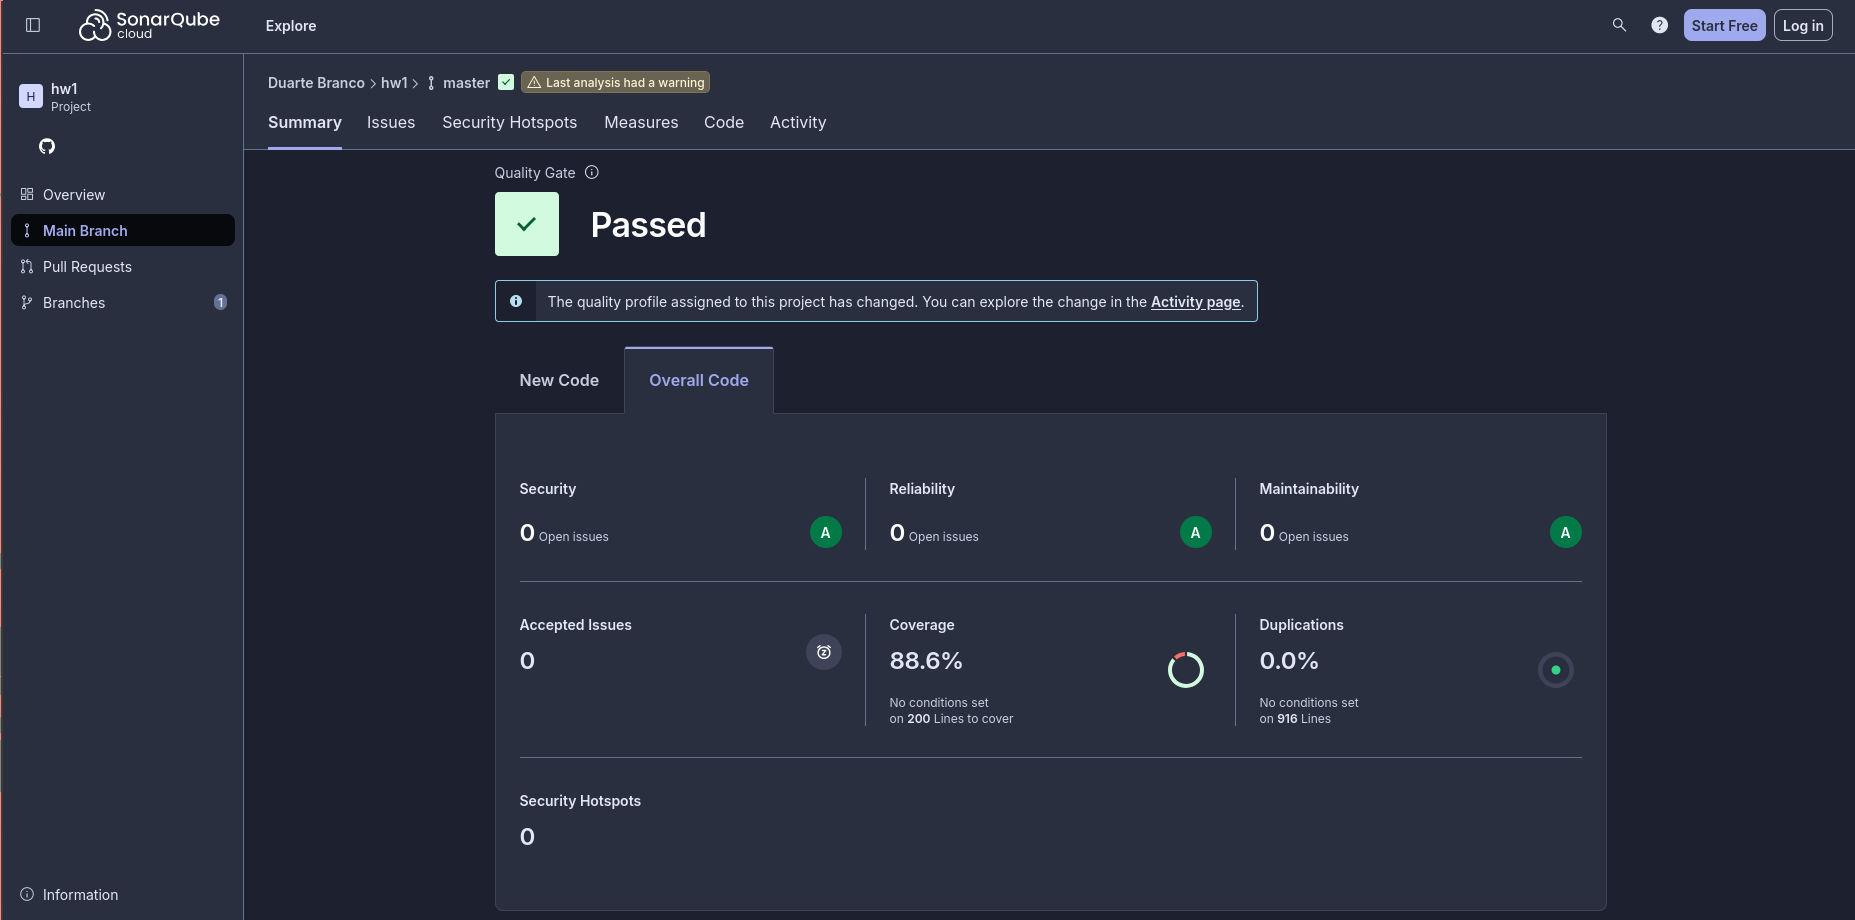
\includegraphics[width=0.8\textwidth]{images/sonarqube.png}
    \caption{\texttt{SonarQube} dashboard}
	\label{fig:sonarqube}
\end{figure}

\section{Continuous integration pipeline}

A full continuous integration (CI) workflow was implemented using \textbf{GitHub Actions}, defined in \texttt{ci.yml}. The pipeline runs automatically on every push and pull request to the repository, enforcing build integrity, test execution, and code quality checks.

The CI workflow includes the following stages:

\begin{enumerate}
  \item \textbf{Environment Setup:} A \texttt{PostgreSQL} service is launched in Docker using GitHub-hosted runners. The Spring Boot application connects to this database during test execution.
  \item \textbf{Readiness check:} A manual loop using \texttt{nc -z localhost 5432} ensures PostgreSQL is reachable before proceeding with the build.
  \item \textbf{Build and static analysis:} The Maven build uses \texttt{clean verify} to compile and test the project. Immediately afterward, the \texttt{sonar-maven-plugin} uploads coverage and static analysis metrics to \textbf{SonarCloud}.
  \item \textbf{Quality Gate enforcement:} The job waits for the SonarCloud Quality Gate result using the \texttt{sonarsource/sonarqube-quality-gate-action}. If the gate is not passed (e.g., low coverage, code smells, or vulnerabilities), the workflow fails and the pull request is blocked.
\end{enumerate}

This pipeline ensures that only clean, tested, and maintainable code is merged into the main branch. It also provides fast feedback to developers by catching regressions and enforcing standards at every commit.

\chapter{References \& resources}

\begin{itemize}
	\item \textbf{Video demo}: \texttt{/docs/demo.mp4}
	\item \href{https://github.com/duartebranco/ZeroMonos}{\textbf{Public Repository} (for \textit{SonarQube Cloud} to work)}
	\item \href{https://sonarcloud.io/summary/overall?id=duartebranco\_ZeroMonos\&branch=master}{\textbf{Quality Gate dashboard}}
\end{itemize}

\end{document}
